%%
%% This is file `mcmthesis-demo.tex',
%% generated with the docstrip utility.
%%
%% The original source files were:
%%
%% mcmthesis.dtx  (with options: `demo')
%%
%% -----------------------------------
%%
%% This is a generated file.
%%
%% Copyright (C)
%%       2010 -- 2015 by Zhaoli Wang
%%       2014 -- 2019 by Liam Huang
%%       2019 -- present by latexstudio.net
%%
%% This work may be distributed and/or modified under the
%% conditions of the LaTeX Project Public License, either version 1.3
%% of this license or (at your option) any later version.
%% The latest version of this license is in
%%   http://www.latex-project.org/lppl.txt
%% and version 1.3 or later is part of all distributions of LaTeX
%% version 2005/12/01 or later.
%%
%% This work has the LPPL maintenance status `maintained'.
%%
%% The Current Maintainer of this work is Liam Huang.
%%
%%
%% This is file `mcmthesis-demo.tex',
%% generated with the docstrip utility.
%%
%% The original source files were:
%%
%% mcmthesis.dtx  (with options: `demo')
%%
%% -----------------------------------
%%
%% This is a generated file.
%%
%% Copyright (C)
%%       2010 -- 2015 by Zhaoli Wang
%%       2014 -- 2019 by Liam Huang
%%       2019 -- present by latexstudio.net
%%
%% This work may be distributed and/or modified under the
%% conditions of the LaTeX Project Public License, either version 1.3
%% of this license or (at your option) any later version.
%% The latest version of this license is in
%%   http://www.latex-project.org/lppl.txt
%% and version 1.3 or later is part of all distributions of LaTeX
%% version 2005/12/01 or later.
%%
%% This work has the LPPL maintenance status `maintained'.
%%
%% The Current Maintainer of this work is Liam Huang.
%%
\documentclass{mcmthesis}
\mcmsetup{CTeX = false,    % 使用 CTeX 套装时,设置为 true
          tcn = \textcolor{black}{2412209}, problem = \textcolor{black}{C},
          sheet = true, titleinsheet = true, keywordsinsheet = true,
          titlepage = false, abstract = false}
        
\usepackage{newtxtext}     % \usepackage{palatino}
% \usepackage[backend=bibtex]{biblatex}   % for RStudio Complie
\renewcommand\thefootnote{\textcolor{red}{\arabic{footnote}}}

\usepackage{tocloft}
\setlength{\cftbeforesecskip}{6pt} 
\renewcommand{\contentsname}{\hspace*{\fill}\Large\bfseries Contents \hspace*{\fill}}

\title{Enjoy a Cozy and Green Bath}
% \author{\small \href{http://www.latexstudio.net/}
%   {
\includegraphics[width=7cm]{mcmthesis-logo}}}
\date{\today}



\usepackage{enumitem}
\usepackage{cite}
\renewcommand\thefootnote{\textcolor{red}{\arabic{footnote}}}
\usepackage{hyperref}
\hypersetup{ citecolor=blue, urlcolor=blue}

\setlength{\parindent}{0pt} %首行缩进
% \setlength{\parskip}{0.5em} %段间距
% \renewcommand{\baselinestretch}{1} %行距
% \setlength\abovedisplayskip{0pt} %公式前后段间距
% \setlength\belowdisplayskip{0pt}

% \usepackage{geometry}
% \geometry{a4paper,left=2cm,right=2cm,top=2.5cm,bottom=1cm} %页边距



\begin{document}

\begin{abstract}

\begin{keywords}
Heat transfer, Thermodynamic system, CFD, Energy conservation
\end{keywords}

\end{abstract}

\maketitle

%% Generate the Table of Contents, if it's needed.
% \renewcommand{\contentsname}{\centering Contents}
\tableofcontents        % 若不想要目录, 注释掉该句
\thispagestyle{empty}

\newpage

\section{Introduction}

\subsection{Background}

1.1

\subsection{Literature Review}

1.2

\subsection{Restatement of the Problem}


\section{Assumptions and Justification}

To simplify the problem and make it convenient for us to simulate real-life conditions, we make the following basic assumptions, each of which is properly justified.

\begin{itemize}[leftmargin=*]
\end{itemize}

\section{Notations}
\vspace{1em}
\begin{center}
\begin{tabular}{clc}
\toprule
{\bf Symbols} & {\bf Description} & \quad {\bf Unit} \\[0.05cm] 
\midrule
$h$ & Convection heat transfer coefficient & \quad W/(m$^2 \cdot$ K) 
\\[0.2cm]
$k$ & Thermal conductivity & \quad W/(m $\cdot$ K) \\[0.2cm]
$c_p$ & Specific heat & \quad J/(kg $\cdot$ K) \\[0.2cm]
$\rho$ & Density & \quad kg/m$^2$ \\[0.2cm]
$\delta$ & Thickness & \quad m \\[0.2cm]
$t$ & Temperature & \quad $^\circ$C, K \\[0.2cm]
$\tau$ & Time & \quad s, min, h \\[0.2cm]
$q_m$ & Mass flow & \quad kg/s \\[0.2cm]
$\Phi$ & Heat transfer power & \quad W \\[0.2cm]
$T$ & A period of time & \quad s, min, h \\[0.2cm]
$V$ & Volume & \quad m$^3$, L \\[0.2cm]
$M,\,m$ & Mass & \quad kg \\[0.2cm]
$A$ & Aera & \quad m$^2$ \\[0.2cm]
$a,\,b,\,c$ & The size of a bathtub  & \quad m$^3$
\\
\bottomrule
\end{tabular}
\end{center}

\noindent where we define the main parameters while specific value of those parameters will be given later.

\section{Model Overview}

In our basic model, we aim at three goals: keeping the temperature as even as possible, making it close to the initial temperature and decreasing the water consumption.

We start with the simple sub-model where hot water is added constantly.
At first we introduce convection heat transfer control equations in rectangular coordinate system. Then we define the mean temperature of bath water.

Afterwards, we introduce Newton cooling formula to determine heat transfer
capacity. After deriving the value of parameters, we get calculating results via formula deduction and simulating results via CFD.

Secondly, we present the complicated sub-model in which hot water is
added discontinuously. We define an iteration consisting of two process:
heating and standby. As for heating process, we derive control equations and boundary conditions. As for standby process, considering energy conservation law, we deduce the relationship of total heat dissipating capacity and time.

Then we determine the time and amount of added hot water. After deriving the value of parameters, we get calculating results via formula deduction and simulating results via CFD.

At last, we define two criteria to evaluate those two ways of adding hot water. Then we propose optimal strategy for the user in a bathtub.
The whole modeling process can be shown as follows.

\begin{figure}[h] 
\centering
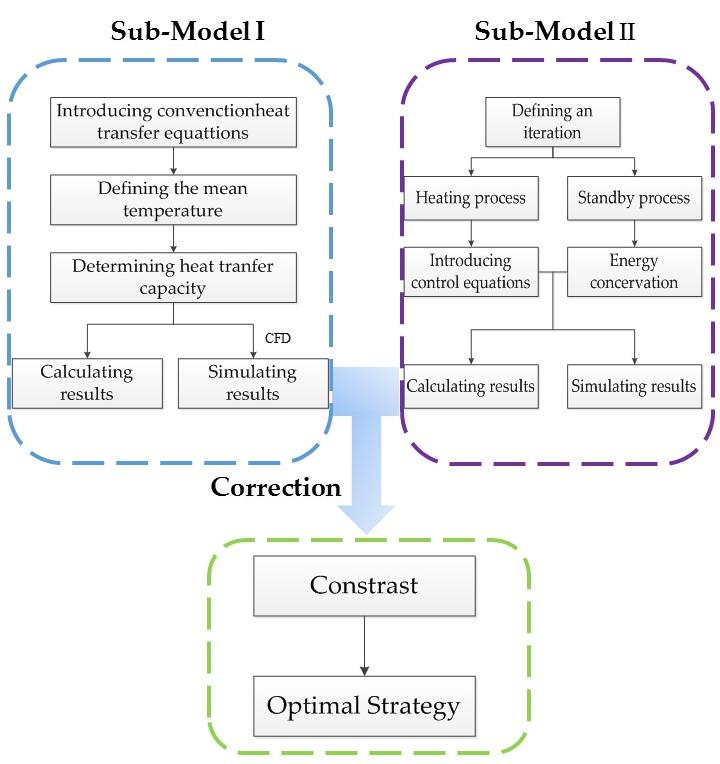
\includegraphics[width=12cm]{fig1.jpg}
\caption{Modeling process} \label{fig1}
\end{figure}


\section{独立性检验}
显然,在影响得分的因素中,选手能力是一个最主要的影响因素,在两两之间的对垒中,单次得分的概率分布取决于选手综合素质的差值. 
但是否每次得分结果都是独立的二项分布,还是存在其他的影响因素影响比赛结果,这是我们需要检验的问题.
具体地,我们考虑了两个方向的检验:
(1) 发球优势是否影响得分结果
(2) 之前的比赛结果是否影响得分结果
To this end, 我们使用了卡方检验\footnote{卡方独立性检验是用于两个或两个以上因素多项分类的计数资料分析,即研究两类变量之间(以列联表形式呈现)的关联性和依存性,或相关性、独立性、交互作用性。}来验证相关性。
考虑两个变量$X$和$Y$,他们的值域分别为$\{x_1,x_2,\cdots,x_m\}$和$\{y_1,y_2,\cdots,y_n\}$,我们可以得到一个列联表,如下所示:
\begin{table}[h]
\centering
\caption{列联表}
\label{tab1}
\begin{tabular}{|c|c|c|c|c|}
\hline
 & $y_1$ & $y_2$ & $\cdots$ & $y_n$ \\ \hline
$x_1$ & $n_{11}$ & $n_{12}$ & $\cdots$ & $n_{1n}$ \\ \hline
$x_2$ & $n_{21}$ & $n_{22}$ & $\cdots$ & $n_{2n}$ \\ \hline
$\vdots$ & $\vdots$ & $\vdots$ & $\ddots$ & $\vdots$ \\ \hline
$x_m$ & $n_{m1}$ & $n_{m2}$ & $\cdots$ & $n_{mn}$ \\ \hline
\end{tabular}
\end{table}
其中,$n_{ij}$表示当$X=x_i$时,$Y=y_j$的频数。我们可以得到如下的假设:
\begin{itemize}
\item $H_0$:$X$和$Y$是独立的
\item $H_1$:$X$和$Y$不是独立的
\end{itemize}
我们可以使用卡方统计量来检验这个假设:
\begin{equation*}
\chi^2 = \sum_{i=1}^m\sum_{j=1}^n\frac{(n_{ij}-E_{ij})^2}{E_{ij}}
\end{equation*}
其中,$E_{ij}$是$X=x_i$和$Y=y_j$的期望频数, $chi^2$的值越大,我们越有理由拒绝$H_0$,即$X$和$Y$不是独立的。

\textbf{验证发球优势与得分的相关性} 
    我们设置$X$为是否发球,$Y$ 为是否得分,然后使用卡方检验来验证发球优势是否影响得分结果。
    我们分别使用了所有比赛数据的得分情况以及在每一场比赛的得分情况来进行检验,结果如图fig~\ref{}
    fig~\ref{}.a 表示是否发球和是否得分的连列表,这里包含了每一场比赛的数据。我们可以看到,卡方统计量的值为1556.61,显著性p近似于,所以我们拒绝了$H_0$,即发球优势与得分结果是有相关性的。
    fig~\ref{}.b 中进一步验证每一场比赛中发球优势与得分的相关性, 可见几乎每一场比赛的卡方统计量都是显著的。

\textbf{验证之前比赛结果与得分的相关性}
    
\textbf{\textit{去除发球的影响,动量与得分仍呈现出相关性}}



\section{模型建立}

对于每一个point,我们使用胜率p来衡量选手的表现,即选手在此point下胜负结果服从参数为p的0-1分布,通过极大似然估计可以从已有数据得到真实分布的p,而极大似然等价于最小化KL散度,故可由此将KL散度发展为评估模型的指标,即观察我们建模出的p与真实p之间的差异。



\subsection{Model \uppercase\expandafter{\romannumeral1}: Bradley-Terry模型}

对于如何建模出p,由于此温网比赛为32强淘汰赛,32位选手共打了31场比赛,我们可以通过这31场比赛的结果来估计每位选手的p,我们使用Bradley-Terry模型来建模p。


\subsubsection{based Bradley-Terry模型}

设有 $n$ 个个体 $\{1,2, \cdots, n\}$ 进行两两比较, 将个体 $k$ 的能力参数记为 $\beta_k(k=1,2, \cdots, n), P_{k, j}$ 表示个体 $k$ 的能力优于个体 $j$ 的概率, B-T 模型将概率表示为
\begin{equation*}
P_{k, j}=\exp \left(\beta_k-\beta_j\right) /\left[1+\exp \left(\beta_k-\beta_j\right)\right],
\end{equation*}
$P_{k, j}$ 只依赖 $\beta_k$ 与 $\beta_j$ 之差.
假设 $N_{k j}$ 表示个体 $k$ 和个体 $j$ 之间进行比较的总次数, 其中, 个体 $k$ 优于个体 $j$ 的次数为 $n_{k j}$, 个体 $j$ 优于个体 $k$ 的次数为 $n_{j k}=N_{k j}-n_{k j}$, 则关于个体能力参数 $\beta_k(k=1,2, \cdots, n)$ 的似然函数为
\begin{equation*}
L\left(\beta_1, \beta_2, \cdots, \beta_n\right)=\prod_{1 \leqslant k \neq j \leqslant n} \frac{N_{k j} !}{n_{k j} !\left(N_{k j}-n_{k j}\right) !}\left(\frac{\exp \left(\beta_k-\beta_j\right)}{1+\exp \left(\beta_k-\beta_j\right)}\right)^{n_{k j}}\left(\frac{1}{1+\exp \left(\beta_k-\beta_j\right)}\right)^{\left(N_{k j}-n_{k j}\right)} .
\end{equation*}

考虑到模型的可识别性, 模型的约束条件为 $\sum_{k=1}^n \beta_k=0$, 或者某个 $\beta_k=0, k \in\{1,2, \cdots, n\}$.


\subsubsection{Bradley-Terry模型 with 发球因素}

在网球比赛中, $h$ 表示发球方, $v$ 表示接球方, 在第 $i$ 场比赛中, 只有胜、负两种比赛结果, 若发球方胜,记为 $Y_i=1$, 否则为 $Y_i=0$. 如果考虑主场因素, 需要把所有球队主场参数 $\delta$ 加人到 B-T 模型 (1) 中, 模型为
\begin{equation*}
P\left(Y_i=1\right)=\exp \left(\delta+\beta_{h_i}-\beta_{v_i}\right) /\left[1+\exp \left(\delta+\beta_{h_i}-\beta_{v_i}\right)\right] .
\end{equation*}

对模型参数极大似然估计时, 似然函数式 (2) 也作相应的修改.




\subsection{Model \uppercase\expandafter{\romannumeral2}: 动态 B-T 模型}

\subsubsection{ 基于马尔可夫过程的动态 B-T 模型}




\subsubsection{ 基于 EWMA 过程的动态 B-T 模型}

在赛季期间, 由于球员会受到伤病、心理、疲劳等各种因素影响, 球队比赛的实力会发生变化, 因此考虑在 $\mathrm{B}-\mathrm{T}$ 模型中引人 EWMA 过程, 动态评估各支球队的实力.
设 $\beta_{h_i}\left(t_i\right)$ 表示 $t_i$ 时间第 $i$ 场比赛主队 $h_i$ 的实力, 通过 EWMA 过程可得
\begin{equation*}
\beta_{h_i}\left(t_i\right)=\alpha_1 \lambda_1 r_{h_i}\left(t_i^{(-1)}\right)+\left(1-\lambda_1\right) \beta_{h_i}\left(t_i^{(-1)}\right) .
\end{equation*}

其中, $\alpha_1$ 是主场参数, $\lambda_1 \in[0,1]$ 是主场平滑参数, $r_{h_1}\left(t_i^{(-1)}\right)$ 是主队 $h_i$ 在时间 $t_i^{(-1)}$ 时比赛结果变量.
此外用式 4) 计算时需要一个迭代计算的初始值, 记为 $\alpha_1 \bar{r}_h$, 其中, $\bar{r}_h$ 可以取主队之前比赛结果的平均值. 假设主场球队 $h_i$ 在时间 $t_i$ 时已进行了 $K$ 场主场比赛, 由式 (4) 可得
\begin{equation*}
\beta_{h_i}\left(t_i\right)=\alpha_1\left\{\lambda_1 \sum_{k=0}^{K-1}\left(1-\lambda_1\right)^k r_{h_i}\left(t_i^{(-k-1)}\right)+\left(1-\lambda_1\right)^K \bar{r}_h\right\}=\alpha_1 x_{h_i}\left(t_i ; \lambda_1\right) .
\end{equation*}

因此, $\beta_{h_i}\left(t_i\right)$ 表示主队之前全部比赛结果 $r_{h_i}\left(t_i^{(-1)}\right), r_{h_i}\left(t_i^{(-2)}\right), \cdots, r_{h_i}\left(t_i^{(-K)}\right)$ 的函数.
同理, 客场实力 $\beta_{v_i}\left(t_i\right)$ 可表示为
\begin{equation*}
\beta_{v_i}\left(t_i\right)=\alpha_2\left\{\lambda_1 \sum_{k=0}^{K-1}\left(1-\lambda_2\right)^k r_{v_i}\left(t_i^{(-k-1)}\right)+\left(1-\lambda_2\right)^K \bar{r}_v\right\}=\alpha_2 x_{v_i}\left(t_i ; \lambda_2\right) .
\end{equation*}

再将式 (5) 和式 (6) 代人式 (3), 模型改为
\begin{equation*}
P\left(Y_i=y_i \mid Y_{i-1}=y_{i-1}, \cdots, Y_1=y_1\right)=\frac{\exp \left\{\delta_{y_i}+\beta_{h_i}\left(t_i\right)-\beta_{v_i}\left(t_i\right)\right.}{1+\exp \left\{\delta_{y_i}+\beta_{h_i}\left(t_i\right)-\beta_{v_i}\left(t_i\right)\right\}} .
\end{equation*}

称为动态的 $\mathrm{B}-\mathrm{T}$ 模型.
设模型的迭代参数为 $\gamma=\left(\alpha_1, \alpha_2, \delta\right)^{\mathrm{T}}$, 平滑参数为 $\lambda=\left(\lambda_1, \lambda_2\right)^{\mathrm{T}}$, 记 $\theta=\left(\gamma^{\mathrm{T}}, \lambda^{\mathrm{T}}\right)^{\mathrm{T}}$, 相应地, 式 (7) 表示为
\begin{equation*}
P\left(Y_i=y_i \mid Y_{i-1}=y_{i-1}, \cdots, Y_1=y_1 ; \theta\right)=\frac{\exp \left\{\delta_{y_i}+\alpha_1 x_{h_i}\left(t_i ; \lambda_1\right)-\alpha_2 x_{v_i}\left(t_i ; \lambda_2\right)\right\}}{1+\exp \left\{\delta_{y_i}+\alpha_1 x_{h_i}\left(t_i ; \lambda_1\right)-\alpha_2 x_{v_i}\left(t_i ; \lambda_2\right)\right\}} .
\end{equation*}

模型参数的似然函数为
\begin{equation*}
L(\theta ; y)=P\left(Y_1=y_1 ; \theta\right) \prod_{i=2}^n P\left(Y_i=y_i \mid Y_{i-1}=y_{i-1}, \cdots, Y_1=y_1 ; \theta\right) .
\end{equation*}




\section{Sub-model II: }

In order to establish the unsteady sub-model, we recall on the working principle of air conditioners. The heating performance of air conditions consist of two processes: heating and standby. After the user set a temperature, the air conditioner will begin to heat until the expected temperature is reached. Then it will go standby. When the temperature get below the expected temperature, the air conditioner begin to work again. As it works in this circle, the temperature remains the expected one.

Inspired by this, we divide the bathtub working into two processes: adding
hot water until the expected temperature is reached, then keeping this
condition for a while unless the temperature is lower than a specific value. Iterating this circle ceaselessly will ensure the temperature kept relatively stable.

\subsection{Heating Model}

\subsubsection{Control Equations and Boundary Conditions}

\subsubsection{Determination of Inflow Time and Amount}

\subsection{Standby Model}

\subsection{Results}

\quad~ We first give the value of parameters based on others’ studies. Then we get the calculation results and simulating results via those data.

\subsubsection{Determination of Parameters}

After establishing the model, we have to determine the value of some
important parameters.

As scholar Beum Kim points out, the optimal temperature for bath is
between 41 and 45$^\circ$C [1]. Meanwhile, according to Shimodozono's study, 41$^\circ$C warm water bath is the perfect choice for individual health [2]. So it is reasonable for us to focus on $41^\circ$C $\sim 45^\circ$C. Because adding hot water continuously is a steady process, so the mean temperature of bath water is supposed to be constant. We value the temperature of inflow and outflow water with the maximum and minimum temperature respectively.

The values of all parameters needed are shown as follows:

.....

\subsubsection{Calculating Results}

Putting the above value of parameters into the equations we derived before, we can get the some data as follows:

%%普通表格
\begin{table}[h]  %h表示固定在当前位置
\centering        %设置居中
\caption{The calculating results}  %表标题
\vspace{0.15cm}
\label{tab2}                       %设置表的引用标签
\begin{tabular}{|c|c|c|}  %3个c表示3列, |可选, 表示绘制各列间的竖线
\hline                    %画横线
Variables & Values & Unit     \\ \hline  %各列间用&隔开
$A_1$     & 1.05   &   $m^2$  \\ \hline
$A_2$     & 2.24   &   $m^2$  \\ \hline
$\Phi_1$  & 189.00 &   $W$   \\ \hline
$\Phi_2$  & 43.47  &   $W$   \\ \hline
$\Phi$    & 232.47 &   $W$   \\ \hline
$q_m$     & 0.014  &   $g/s$ \\ \hline
\end{tabular}
\end{table}

From Table \ref{tab2}, ......

......

\section{Correction and Contrast of Sub-Models}

After establishing two basic sub-models, we have to correct them in consideration of evaporation heat transfer. Then we define two evaluation criteria to compare the two sub-models in order to determine the optimal bath strategy.

\subsection{Correction with Evaporation Heat Transfer}

Someone may confuse about the above results: why the mass flow in the first sub-model is so small? Why the standby time is so long? Actually, the above two sub-models are based on ideal conditions without consideration of the change of boundary conditions, the motions made by the person in bathtub and the evaporation of bath water, etc. The influence of personal motions will be discussed later. Here we introducing the evaporation of bath water to correct sub-models.

\subsection{Contrast of Two Sub-Models}

Firstly we define two evaluation criteria. Then we contrast the two submodels via these two criteria. Thus we can derive the best strategy for the person in the bathtub to adopt.

\section{Model Analysis and Sensitivity Analysis}

\subsection{The Influence of Different Bathtubs}

Definitely, the difference in shape and volume of the tub affects the
convection heat transfer. Examining the relationship between them can help
people choose optimal bathtubs.

\subsubsection{Different Volumes of Bathtubs}

In reality, a cup of water will be cooled down rapidly. However, it takes quite long time for a bucket of water to become cool. That is because their volume is different and the specific heat of water is very large. So that the decrease of temperature is not obvious if the volume of water is huge. That also explains why it takes 45 min for 320 L water to be cooled by 1$^\circ$C.

In order to examine the influence of volume, we analyze our sub-models
by conducting sensitivity Analysis to them.

We assume the initial volume to be 280 L and change it by $\pm 5$\%, $\pm 8$\%, $\pm 12$\% and $\pm 15$\%. With the aid of sub-models we established before, the variation of some parameters turns out to be as follows

%%三线表
\begin{table}[h] %h表示固定在当前位置
\centering  %设置居中
\caption{Variation of some parameters}  %表标题
\label{tab7} %设置表的引用标签
\begin{tabular}{ccccccc} %7个c表示7列, c表示每列居中对齐, 还有l和r可选
\toprule  %画顶端横线
$V$      & $A_1$   & $A_2$   & $T_2$    & $q_{m1}$ & $q_{m2}$ & $\Phi_q$ \\
\midrule  %画中间横线
-15.00\% & -5.06\% & -9.31\% & -12.67\% & -2.67\%  & -14.14\% & -5.80\% \\
-12.00\% & -4.04\% & -7.43\% & -10.09\% & -2.13\%  & -11.31\% & -4.63\% \\
-8.00\%  & -2.68\% & -4.94\% & -6.68\%  & -1.41\%  & -7.54\%  & -3.07\% \\
-8.00\%  & -2.68\% & -4.94\% & -6.68\%  & -1.41\%  & -7.54\%  & -3.07\% \\
-8.00\%  & -2.68\% & -4.94\% & -6.68\%  & -1.41\%  & -7.54\%  & -3.07\% \\
-8.00\%  & -2.68\% & -4.94\% & -6.68\%  & -1.41\%  & -7.54\%  & -3.07\% \\
-8.00\%  & -2.68\% & -4.94\% & -6.68\%  & -1.41\%  & -7.54\%  & -3.07\% \\
-8.00\%  & -2.68\% & -4.94\% & -6.68\%  & -1.41\%  & -7.54\%  & -3.07\% \\
-8.00\%  & -2.68\% & -4.94\% & -6.68\%  & -1.41\%  & -7.54\%  & -3.07\% \\
-8.00\%  & -2.68\% & -4.94\% & -6.68\%  & -1.41\%  & -7.54\%  & -3.07\% \\
-8.00\%  & -2.68\% & -4.94\% & -6.68\%  & -1.41\%  & -7.54\%  & -3.07\% \\
\bottomrule  %画底部横线
\end{tabular}
\end{table}

\section{Strength and Weakness}

\subsection{Strength}

\begin{itemize}[leftmargin=*]
\item We analyze the problem based on thermodynamic formulas and laws, so that the model we established is of great validity.

\item Our model is fairly robust due to our careful corrections in consideration of real-life situations and detailed sensitivity analysis.

\item Via Fluent software, we simulate the time field of different areas throughout the bathtub. The outcome is vivid for us to understand the changing process.

\item We come up with various criteria to compare different situations, like water consumption and the time of adding hot water. Hence an overall comparison can be made according to these criteria.

\item Besides common factors, we still consider other factors, such as evaporation and radiation heat transfer. The evaporation turns out to be the main reason of heat loss, which corresponds with other scientist’s experimental outcome.
\end{itemize}

\subsection{Weakness}

\begin{itemize}[leftmargin=*]
\item Having knowing the range of some parameters from others’ essays, we choose a value from them to apply in our model. Those values may not be reasonable in reality.

\item Although we investigate a lot in the influence of personal motions, they are so complicated that need to be studied further.

\item Limited to time, we do not conduct sensitivity analysis for the influence of personal surface area.
\end{itemize}

\section{Further Discussion}

In this part, we will focus on different distribution of inflow faucets. Then we discuss about the real-life application of our model.

\begin{itemize}[leftmargin=*]
\item Different Distribution of Inflow Faucets

In our before discussion, we assume there being just one entrance of inflow.

From the simulating outcome, we find the temperature of bath water is hardly even. So we come up with the idea of adding more entrances.

The simulation turns out to be as follows

\begin{figure}[h] 
\centering
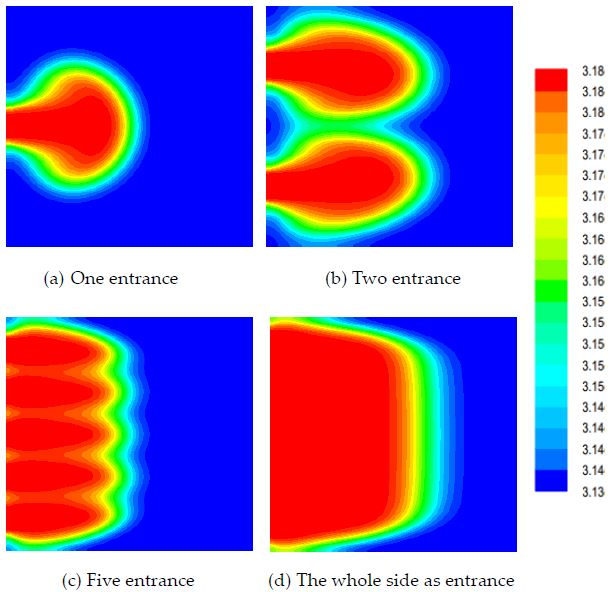
\includegraphics[width=12cm]{fig24.jpg}
\caption{The simulation results of different ways of arranging entrances} \label{fig24}
\end{figure}

From the above figure, the more the entrances are, the evener the temperature will be. Recalling on the before simulation outcome, when there is only one entrance for inflow, the temperature of corners is quietly lower than the middle area.

In conclusion, if we design more entrances, it will be easier to realize the goal to keep temperature even throughout the bathtub.

\item Model Application

Our before discussion is based on ideal assumptions. In reality, we have to make some corrections and improvement.

\begin{itemize}[leftmargin=*]
\item[1)] Adding hot water continually with the mass flow of 0.16 kg/s. This way can ensure even mean temperature throughout the bathtub and waste less water.

\item[2)] The manufacturers can design an intelligent control system to monitor the temperature so that users can get more enjoyable bath experience.

\item[3)] We recommend users to add bubble additives to slow down the water being cooler and help cleanse. The additives with lower thermal conductivity are optimal.

\item[4)] The study method of our establishing model can be applied in other area relative to convection heat transfer, such as air conditioners.
\end{itemize}
\end{itemize}

\bibliographystyle{unsrt}
\bibliography{reference}


\newpage

\begin{letter}{Enjoy Your Bath Time!}

From simulation results of real-life situations, we find it takes a period of time for the inflow hot water to spread throughout the bathtub. During this process, the bath water continues transferring heat into air, bathtub and the person in bathtub. The difference between heat transfer capacity makes the temperature of various areas to be different. So that it is difficult to get an evenly maintained temperature throughout the bath water.

In order to enjoy a comfortable bath with even temperature of bath water and without wasting too much water, we propose the following suggestions.

\begin{itemize}[leftmargin=*]
\item Adding hot water consistently
\item Using smaller bathtub if possible
\item Decreasing motions during bath
\item Using bubble bath additives
\item Arranging more faucets of inflow
\end{itemize}

\vspace{\parskip}

Sincerely yours,

Your friends

\end{letter}

\newpage

\begin{appendices}

\section{First appendix}

In addition, your report must include a letter to the Chief Financial Officer (CFO) of the Goodgrant Foundation, Mr. Alpha Chiang, that describes the optimal investment strategy, your modeling approach and major results, and a brief discussion of your proposed concept of a return-on-investment (ROI). This letter should be no more than two pages in length.

Here are simulation programmes we used in our model as follow.\\

\textbf{\textcolor[rgb]{0.98,0.00,0.00}{Input matlab source:}}
\lstinputlisting[language=Matlab]{./code/mcmthesis-matlab1.m}

\section{Second appendix}

some more text \textcolor[rgb]{0.98,0.00,0.00}{\textbf{Input C++ source:}}
\lstinputlisting[language=C++]{./code/mcmthesis-sudoku.cpp}

\end{appendices}

\newpage
\newcounter{lastpage}
\setcounter{lastpage}{\value{page}}
\thispagestyle{empty} 

\section*{Report on Use of AI}

This report aims to provide a detailed explanation of the AI techniques we utilized during the MCM/ICM mathematical modeling competition and elucidate their advantages and disadvantages, as well as their application in our modeling and analysis process.

\subsection*{Utilized AI Techniques}

The following AI techniques were employed during our modeling and analysis:

\begin{itemize}[leftmargin=*]
\item Neural Networks
\item Decision Trees
\item Cluster Analysis
\end{itemize}

Neural networks were used to predict trends and changes related to the problem under investigation, decision trees were utilized to determine correlations between factors, and cluster analysis was applied to identify patterns within the dataset.

\subsection*{Application of Techniques}

For each technique, we elaborate on their pros and cons and justify our decision for selecting these particular methods. Additionally, we outline the approaches and strategies we implemented for data preprocessing, feature engineering, model training, and tuning.

\subsection*{Results and Conclusions}

Using AI techniques, we derived a series of results and conclusions regarding the problem at hand. We evaluated the reliability and accuracy of these outcomes. Through our analysis, we arrived at the following conclusions:

Conclusion 1
Conclusion 2
...

\subsection*{Discussion}

We discuss the future prospects and trends of these techniques, highlighting potential limitations and challenges. Furthermore, we present suggestions and future research directions.

\subsection*{Summary}

This report comprehensively outlines the AI techniques employed during the MCM/ICM competition, detailing their application, obtained results and conclusions, and future research directions. We hope this report serves as a valuable reference for understanding the utilization of AI techniques in modeling and analysis.

% 重置页码
\clearpage
\setcounter{page}{\value{lastpage}}

\end{document}
%%
%% This work consists of these files mcmthesis.dtx,
%%                                   figures/ and
%%                                   code/,
%% and the derived files             mcmthesis.cls,
%%                                   mcmthesis-demo.tex,
%%                                   README,
%%                                   LICENSE,
%%                                   mcmthesis.pdf and
%%                                   mcmthesis-demo.pdf.
%%
%% End of file `mcmthesis-demo.tex'.
